\chapter{Rationality and Intelligence}
\label{sec:p19-rationality-15-2}

An intelligence score and a judgment about rational thinking need not assess
the same thing. Stanovich, Toplak and West's chapter~15.2 compares them as
individual-difference constructs in cognitive science. It adopts a grounded
account of what intelligence tests measure, then argues that rational
responding additionally depends on dispositions to initiate reflection and
on learned knowledge and strategies. Its tripartite architecture explains
how substantial computational ability can coexist with poorly supported
beliefs or injudicious decisions
\cite[pp.~791--800]{StanovichToplakWest2021Intelligence}.

This is a specified psychological comparison, not a universal definition of
rationality, an assessment of someone's worth, or a diagnostic rule derived
from an IQ score. The source reconstructs a cognitive architecture and
reviews qualitative individual-difference findings. It does not provide
participant-level methods, correlation tables or a standardized rationality
test with a complete scoring manual in this chapter. Its four figures are
functional models, not measured maps of three anatomically separate modules.

\section{Match the construct to its measurement}
\label{sec:p19-rat152-constructs}

\begin{hbdefinition}{def:p19-rat152-grounding}{Grounded intelligence and individual-difference rationality}
A permissive conception of intelligence includes whatever the broad everyday
word suggests, such as adaptation, wisdom or creativity, whether or not
existing IQ tests measure those capacities. The source's grounded conception
instead anchors intelligence to the abilities assessed by the tests being
discussed. In the Cattell--Horn--Carroll account, general intelligence is
conventionally denoted \(g\), with broad factors including fluid and
crystallized intelligence.

Fluid intelligence concerns reasoning across domains, including unfamiliar
ones; the chapter names figural analogies, Raven matrices and series
completion as measurement families. Crystallized intelligence concerns
knowledge acquired through acculturated learning; vocabulary, verbal
comprehension and general knowledge are its named measurement families.
These names identify constructs and task families, not a locally supplied
test battery or interchangeable measures of every reasoning skill.

Rationality in this comparison concerns individual differences in responses
evaluated against stated normative models. The relevant departure is from
the specified model's standard, not from a researcher's personal preference.
The concept must be assessed at a grain comparable to the individual-difference
concept of intelligence. An all-or-nothing philosophical attribution of
rational agency answers a different question.
\index{intelligence!rationality distinction}
\index{rationality!individual differences}
\index{mindware}
\end{hbdefinition}

The source opens with the apparent paradox of someone described as smart
acting foolishly. If both words refer to intellectual capacity, the phrase
appears contradictory. If the second description instead concerns poor
decisions or careless errors, it distinguishes capacity from judicious
deployment. The dictionary illustration identifies an ambiguity; it does
not supply an empirical frequency of high-IQ mistakes. Adopting a broad
definition that includes wise decisions does not make an existing IQ test
measure that additional property
\cite[secs.~1--2, pp.~791--792]{StanovichToplakWest2021Intelligence}.

The authors characterize CHC as a well-supported grounded framework and
argue that fluid and crystallized abilities leave important rationality
components unmeasured. This is their theoretical and measurement claim,
not the proposition that intelligence is unrelated to reasoning performance.
Test labels alone also do not show that a score is a pure measure of one
process: language, schooling, prior exposure, motivation, task instructions
and measurement error can affect an observed score. Such influences must
be investigated rather than inferred away by calling a test an ability test.

\section{Normative standards and task-specific scoring}
\label{sec:p19-rat152-benchmarks}

The chapter distinguishes epistemic rationality, concerning how beliefs
match the world, from instrumental rationality, concerning achieving one's
goals with the available physical and mental resources. Its more formal
instrumental comparison is expected-utility maximization: weight each
possible outcome's utility by its probability and add the products.
Direct experimental assessment is difficult when personal probabilities
and utilities are hard to elicit. The axiomatic alternative evaluates
patterns of preference against conditions that support an as-if utility
representation \cite[p.~792]{StanovichToplakWest2021Intelligence}.

That representation requires the actual preference domain and axioms.
\Cref{sec:p17-finite-expected-utility} supplies a complete finite-prize
lottery representation under its mixture, continuity and preference
assumptions; the simpler ordinal theorem on a finite set is not sufficient
for all those lottery comparisons. An as-if representation is not a proof
that someone consciously multiplied utilities, a warrant for arbitrary
payoff assignments, or a guarantee of favorable realized outcomes. A
chance outcome can be unlucky after a choice maximizing the stipulated
expected value.

The source's operational task families include probability assessment,
hypothesis testing, utility-axiom consistency, calibration, resistance
to irrelevant contextual influences and consideration of an alternative
hypothesis. The heuristics-and-biases tradition supplies many of those
operationalizations. They can draw on cognitive capacity without exhausting
what an IQ test measures. Their responses also require the relevant learned
knowledge, interpretation and opportunity to apply it.

\begin{hbexample}{def:p19-rat152-scoring-contrast}{Different measures require different criteria}
A figural-analogy item can be scored against its designated completion
rule under instructions to find the correct option. A probability judgment
instead requires a specified event and interpretation; a calibration
judgment additionally requires a collection or law relating reports to
outcomes. As \cref{def:p19-calibration-law} shows, correctness of selected
answers and calibration of confidence are not the same score.

Similarly, a changed preference between two descriptions of the same lottery
is a framing inconsistency only if the descriptions preserve all consequences
and probabilities relevant to the comparison. If one changes information,
timing, social consequences or costs that matter to the person, the premise
of equivalence is not established. A hypothesis-testing answer needs its
alternative hypotheses and the aim of the test specified before it is
called inefficient.

These are stipulated scoring contrasts based on the source's actual task
families, not a newly validated psychometric scale. They do not permit
adding an analogy score, a confidence error and a preference violation
into one rationality quotient without a justified measurement model.
\end{hbexample}

The chapter describes degrees of rationality in terms of distance from a
normative optimum but supplies no single distance function, common unit,
item weighting or population norm covering all these tasks. A proportion
of answers matching a key, a calibration score and a choice-axiom violation
therefore retain their own interpretation. The theoretical argument that
rationality can be measured does not itself provide a complete instrument
or a legitimate threshold for classifying individuals.

\section{The preliminary dual-process architecture}
\label{sec:p19-rat152-dual}

\begin{hbdefinition}{def:p19-rat152-process-types}{Autonomy, override and cognitive decoupling}
In the source's Type~1/Type~2 terminology, autonomy is the defining feature
of Type~1 processing: encountering its triggering conditions initiates it
without a high-level control instruction. Rapid, associative, low-central-load
processing commonly accompanies autonomy but does not define the category.
Many autonomous processes can operate in parallel. Mandatory triggering
does not mean that the resulting response must be emitted without override.

Type~2 processing is nonautonomous and comparatively demanding, with largely
serial use of central resources. It can interrupt a Type~1 response and
simulate an alternative. Cognitive decoupling keeps a hypothetical situation
distinct from the represented actual world while the simulation proceeds.
Representing a premise for purposes of reasoning is not necessarily believing
that premise true of the world.
\end{hbdefinition}

The chapter's preliminary model gives Type~2 a response path and a simulation
path, while Type~1 has its own response path. Preattentive Type~1 computations
also supply input to Type~2. Figure~\ref{fig:p19-rat152-preliminary}
re-presents those source connections. The presence of an override route
does not entail that the autonomous proposal is always wrong. A heuristic
can be adaptive in an environment with suitable cues and costly in an
environment where those cues mislead
\cite[sec.~3, pp.~792--794, fig.~15.2.1]{StanovichToplakWest2021Intelligence}.

\begin{figure}[htbp]
\centering
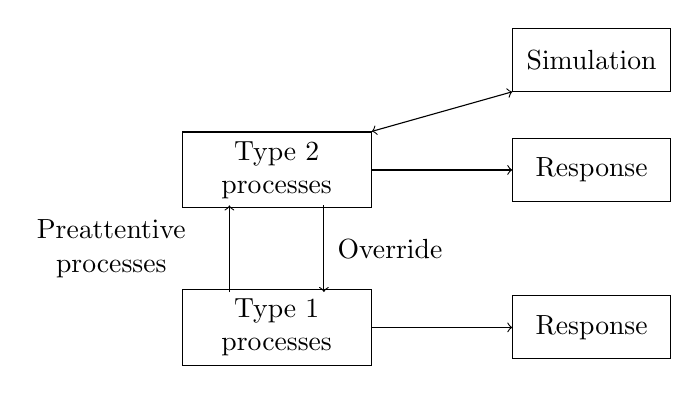
\begin{tikzpicture}[x=1cm,y=1cm]
\node[draw,minimum width=2.4cm,minimum height=.9cm,align=center] (t2) at (0,2) {Type 2\\processes};
\node[draw,minimum width=2.4cm,minimum height=.9cm,align=center] (t1) at (0,0) {Type 1\\processes};
\node[draw,minimum width=2cm,minimum height=.8cm] (sim) at (4,3.4) {Simulation};
\node[draw,minimum width=2cm,minimum height=.8cm] (r2) at (4,2) {Response};
\node[draw,minimum width=2cm,minimum height=.8cm] (r1) at (4,0) {Response};
\draw[<->] (t2.north east)--(sim.south west);
\draw[->] (t2.east)--(r2.west);
\draw[->] (t1.east)--(r1.west);
\draw[->] (-.6,.45)--(-.6,1.55);
\node[align=center] at (-2.1,1) {Preattentive\\processes};
\draw[->] (.6,1.55)--(.6,.45);
\node[right] at (.65,1) {Override};
\end{tikzpicture}
\caption{Native vector reconstruction of the source's preliminary
dual-process model, Figure~15.2.1. Arrows describe proposed functional
connections, not estimates of process strength, duration or brain location.}
\label{fig:p19-rat152-preliminary}
\end{figure}

The source acknowledges multiple dual-process theories and occasionally
uses the similar System~1/System~2 labels. That terminology must not hide
the heterogeneity of autonomous processes or turn speed into a sufficient
classification rule. \Cref{sec:p19-rationality-2-5} develops the broader
dual-process debate and its task-specific evidence; the present chapter
uses the architecture to distinguish kinds of individual differences.

\section{Two levels within Type 2: ability and disposition}
\label{sec:p19-rat152-tripartite}

\begin{hbdefinition}{def:p19-rat152-levels}{Algorithmic and reflective functions}
The algorithmic mind carries out processing: suppressing a triggered
response, sustaining a decoupled representation and computing an alternative.
The reflective mind initiates and regulates those activities in relation to
goals and epistemic commitments. Possessing an operation and initiating it
when appropriate are different proposed functions.

The chapter links variation in fluid intelligence primarily to algorithmic
processing efficiency and variation in thinking dispositions to reflective
control. Thinking dispositions include actively open-minded thinking,
need for cognition, consideration of future consequences, need for closure
and dogmatism. Those constructs and their directions of desirability must
be assessed using specified instruments; listing them does not provide
their scoring keys.
\end{hbdefinition}

The source's psychometric contrast is between maximal and typical
performance. In a maximal-performance assessment, the task interpretation
and goal are externally specified and the participant is asked to do as well
as possible. In a typical-performance assessment, goal selection and usual
epistemic regulation enter the observed behavior. The authors classify
intelligence/aptitude tests with maximal performance and many rational- or
critical-thinking measures with typical performance. This is a distinction
about assessment demands, not evidence that every aptitude-test response
is unaffected by willingness or that a disposition questionnaire is a
pure measure of behavior.

\begin{figure}[htbp]
\centering
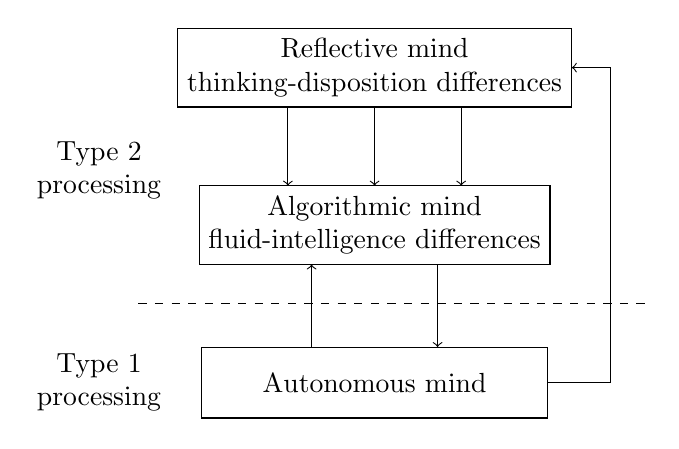
\begin{tikzpicture}[x=1cm,y=1cm]
\node[draw,minimum width=4.4cm,minimum height=1cm,align=center] (ref) at (0,4) {Reflective mind\\thinking-disposition differences};
\node[draw,minimum width=4.4cm,minimum height=1cm,align=center] (alg) at (0,2) {Algorithmic mind\\fluid-intelligence differences};
\node[draw,minimum width=4.4cm,minimum height=.9cm] (aut) at (0,0) {Autonomous mind};
\foreach \x in {-1.1,0,1.1}{\draw[->] (\x,3.5)--(\x,2.5);}
\draw[->] (-.8,.45)--(-.8,1.5);
\draw[->] (.8,1.5)--(.8,.45);
\draw[->] (aut.east)--(3,0)--(3,4)--(ref.east);
\draw[dashed] (-3,1)--(3.5,1);
\node[align=center] at (-3.5,2.7) {Type 2\\processing};
\node[align=center] at (-3.5,0) {Type 1\\processing};
\end{tikzpicture}
\caption{Native reconstruction of Figure~15.2.2. The older Type~1/Type~2
division is the dashed boundary; the added reflective/algorithmic division
is within Type~2. Distinct explanatory roles are not a claim that the
associated measured traits are statistically independent.}
\label{fig:p19-rat152-tripartite}
\end{figure}

Under explicit instructions a participant might correctly compare alternative
hypotheses, yet normally settle on a familiar explanation without making
that comparison. The difference could concern initiation rather than an
inability to perform the operation. Conversely, willingness to reconsider
does not ensure knowledge of the needed rule or sufficient processing
capacity. This is an explanatory contrast permitted by the model, not
an observation of a particular participant's unmeasured mental process.

The source links fluid intelligence, executive function and working memory
to maintaining decoupled simulations. It reports substantial association,
not numerical coefficients or a primary experiment here. A working-memory
score is not direct observation of a decoupling operation. The proposed
link requires a theory connecting the tasks and competing explanations,
not just a shared correlation
\cite[secs.~4--5, pp.~794--795]{StanovichToplakWest2021Intelligence}.

\section{The complete functional model and its limits}
\label{sec:p19-rat152-functions}

The source's Figure~15.2.3 decomposes the routes more precisely. A is
algorithmic override of the autonomous output; B is the reflective
instruction to initiate that override. C is algorithmic decoupling into
simulation; D is the reflective instruction to initiate it. E is serial
associative cognition, and F is a reflective change of control over that
sequence. G denotes preattentive input to higher control. The reflective
initiation calls and the computations they initiate must not be compressed
into one ability variable.

\begin{figure}[htbp]
\centering
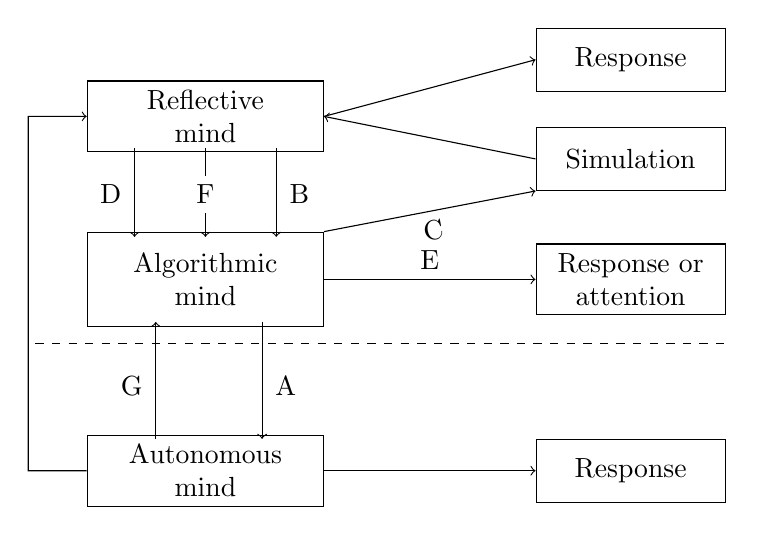
\begin{tikzpicture}[x=1cm,y=1cm,scale=.9]
\node[draw,minimum width=3cm,minimum height=.9cm,align=center] (ref) at (0,5) {Reflective\\mind};
\node[draw,minimum width=3cm,minimum height=1.2cm,align=center] (alg) at (0,2.7) {Algorithmic\\mind};
\node[draw,minimum width=3cm,minimum height=.9cm,align=center] (aut) at (0,0) {Autonomous\\mind};
\node[draw,minimum width=2.4cm,minimum height=.8cm] (rr) at (6,5.8) {Response};
\node[draw,minimum width=2.4cm,minimum height=.8cm] (sim) at (6,4.4) {Simulation};
\node[draw,minimum width=2.4cm,minimum height=.9cm,align=center] (ra) at (6,2.7) {Response or\\attention};
\node[draw,minimum width=2.4cm,minimum height=.8cm] (r1) at (6,0) {Response};
\draw[->] (ref.east)--(rr.west);
\draw[->] (sim.west)--(ref.east);
\draw[->] (alg.north east)--node[below,sloped]{C}(sim.south west);
\draw[->] (alg.east)--node[above]{E}(ra.west);
\draw[->] (aut.east)--(r1.west);
\draw[->] (-1,4.55)--(-1,3.3);
\node[left] at (-1.05,3.9) {D};
\draw[->] (0,4.55)--(0,3.3);
\node[fill=white] at (0,3.9) {F};
\draw[->] (1,4.55)--(1,3.3);
\node[right] at (1.05,3.9) {B};
\draw[->] (-.7,.45)--(-.7,2.1);
\node[left] at (-.75,1.2) {G};
\draw[->] (.8,2.1)--(.8,.45);
\node[right] at (.85,1.2) {A};
\draw[->] (aut.west)--(-2.5,0)--(-2.5,5)--(ref.west);
\draw[dashed] (-2.4,1.8)--(7.4,1.8);
\end{tikzpicture}
\caption{Independent native layout of the complete proposed connections in
Figure~15.2.3, retaining arrows A--G and both autonomous input routes.
The processing/initiating distinction is substantive; node position is
illustrative rather than a neural localization.}
\label{fig:p19-rat152-functions}
\end{figure}

The F instruction can stop a serial association to begin a comprehensive
simulation, or redirect the sequence from another starting point. The
chapter does not develop the full function of serial associative cognition;
it refers to Stanovich's 2011 treatment. An arrow naming that function
does not supply the unprinted complete mechanism. Likewise, the source's
use of hierarchical brain control is a functional explanation, not an
empirical demonstration that each diagram node occupies one brain region
\cite[sec.~6, pp.~795--796]{StanovichToplakWest2021Intelligence}.

\subsection{Mindware and two routes to a normative response}

Perkins's term mindware denotes available learned knowledge, rules,
procedures and strategies used to transform a hypothetical representation.
The chapter emphasizes specialized probabilistic, causal and scientific
knowledge. Ordinary crystallized-intelligence measures broadly sample
vocabulary and general knowledge rather than directly testing all those
specialized resources. A learner can therefore know many words without
knowing an appropriate method for interpreting base rates; knowing the
method also does not ensure applying it.

Some learned rules can become automatic through extensive practice.
Figure~\ref{fig:p19-rat152-mindware} preserves both source routes: accessing
mindware during demanding simulation, and practiced mindware residing
within autonomous processing. Consequently, a response matching a normative
criterion does not uniquely identify Type~2 as its origin. The rule might
have been applied automatically; an erroneous response can instead follow
prolonged deliberate computation with missing or unsuitable knowledge.

\begin{figure}[htbp]
\centering
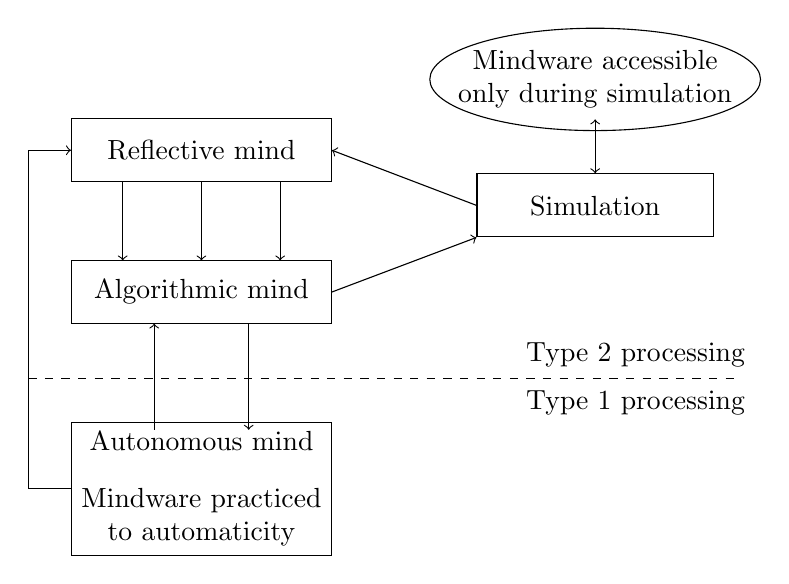
\begin{tikzpicture}[x=1cm,y=1cm]
\node[draw,minimum width=3.3cm,minimum height=.8cm,align=center] (ref) at (0,4.3) {Reflective mind};
\node[draw,minimum width=3.3cm,minimum height=.8cm,align=center] (alg) at (0,2.5) {Algorithmic mind};
\node[draw,minimum width=3.3cm,minimum height=1.5cm,align=center] (aut) at (0,0) {Autonomous mind\\[.3cm]Mindware practiced\\to automaticity};
\node[draw,minimum width=3cm,minimum height=.8cm] (sim) at (5,3.6) {Simulation};
\draw (5,5.2) ellipse (2.1 and .65);
\node[minimum width=3.3cm,minimum height=1cm,align=center] (mw) at (5,5.2) {Mindware accessible\\only during simulation};
\foreach \x in {-1,0,1}{\draw[->] (\x,3.9)--(\x,2.9);}
\draw[->] (-.6,.75)--(-.6,2.1);
\draw[->] (.6,2.1)--(.6,.75);
\draw[->] (aut.west)--(-2.2,0)--(-2.2,4.3)--(ref.west);
\draw[->] (alg.east)--(sim.south west);
\draw[->] (sim.west)--(ref.east);
\draw[<->] (sim.north)--(mw.south);
\draw[dashed] (-2.2,1.4)--(6.8,1.4);
\node[right] at (4,1.7) {Type 2 processing};
\node[right] at (4,1.1) {Type 1 processing};
\end{tikzpicture}
\caption{Native re-presentation of Figure~15.2.4. Autonomous practiced
mindware and simulation-accessible mindware have different routes to
responding. A correct response alone cannot choose between the routes.}
\label{fig:p19-rat152-mindware}
\end{figure}

The source concludes that rational responding can require three classes
of characteristics: computational capacity for override and sustained
simulation, reflective dispositions to initiate useful operations, and
available/accessibly learned mindware, including automatic rules. This is
why its rationality construct is broader than the intelligence construct
it operationalizes. It is not the claim that all three operations occur
in every item or that deliberating longer always improves an answer
\cite[pp.~796--798, fig.~15.2.4]{StanovichToplakWest2021Intelligence}.

\section{Individual-difference claims and their evidence boundary}
\label{sec:p19-rat152-evidence}

The chapter reports that intelligence and thinking dispositions are not
perfectly associated. It describes moderate-to-weak relationships for some
dispositions, including actively open-minded thinking and need for cognition,
and near-zero relationships for others, including conscientiousness,
curiosity and diligence, citing review sources. It further reports that
thinking dispositions predict task variation after general intelligence
is controlled. In this chapter these are qualitative literature reports:
the samples, exact instruments, coefficients, intervals and adjustment
models are not given \cite[sec.~5, p.~795]{StanovichToplakWest2021Intelligence}.

Those claims support the authors' proposal that capacity and regulation
should not be treated as one measured variable. They do not justify
declaring the traits independent, a fixed numerical relation across all
populations, or that an intelligence score predicts a particular person's
judgment. Imperfect measured association can involve measurement error,
restriction of range, differing task demands, prior knowledge or population
selection as well as distinct psychological functions. A residual association
after a selected adjustment is not an experimentally isolated causal effect.

The review's reports about working memory/executive function and its claim
that cognitive ability often, but not always, dissociates from an
evolutionarily characterized modal response have the same source boundary.
No original 1998/1999 dataset or more-than-100-year intelligence history
is reconstructed from a reference citation alone. A strong empirical account
would specify the recruited and analyzed populations, instruction and
scoring versions, repeated observations, reliability, selection, uncertainty
and plausible alternatives, as required by \cref{def:p19-evidence-record}.

\begin{hbwarning}{def:p19-rat152-metric-boundary}{No universal rationality or clinical classification from these diagrams}
Neither \(g\), an IQ score, a thinking-disposition questionnaire nor one
bias task supplies a universal diagnostic measure of rationality. The source's
architectural claims concern specified individual differences and tasks.
They do not license inferring a disorder, fixed incapacity, moral failing
or a population prevalence from an individual answer. A high ability score
does not establish that the relevant reflection occurred; a low score does
not prove that a response violates its stated norm.
\end{hbwarning}

\section{The Great Rationality Debate: what the reconciliation assumes}
\label{sec:p19-rat152-debate}

The authors call one pole Meliorist: observed departures from normative
standards leave room for improvement through education and information.
They call the other Panglossian: the modal response may reflect a suitable
task interpretation or an adaptive information-processing strategy, so
maximal rationality should be a starting presumption. They associate
philosophical, evolutionary, ecological and Bayesian contributions with
the latter pole. These labels organize their debate; they do not show
that every named contributor endorses one identical theory or that every
observed minority answer is normatively better
\cite[sec.~7, pp.~798--799]{StanovichToplakWest2021Intelligence}.

Their proposed reconciliation combines individual-difference patterns with
the differentiated architecture. It distinguishes evolutionary fitness
at the subpersonal genetic level from utility/goal satisfaction at the
personal level. A response favored in an ancestral environment can be
common without best serving an individual's present goals in a different
environment. In the source's proposal, more flexible Type~2 control can
override such a response when the outputs conflict; this makes evolutionary
adaptiveness and personal instrumental or epistemic success different
assessment criteria. References to genes' goals describe an evolutionary
explanatory level, not conscious desires of genes.

The source also invokes a triangulating pattern: higher cognitive ability
is often associated with the response classified as rational for the
individual rather than with the response characterized as evolutionarily
adaptive. It reports exceptions and refers to fuller 1998--2000 studies
and Stanovich's 2004 argument. Those are cited premises of its reconciliation,
not numerical results independently verified here. A response's correlation
with intelligence alone cannot settle the correct normative model; the
model's task interpretation, probabilities, consequences and goals require
their own defense. Nor is ancestral adaptiveness proof of a duty to repeat
the response today.

The architecture itself allows automatic normative mindware and deliberate
error. Therefore its reconciliation cannot consistently be read as
``Type~1 is irrational, Type~2 is rational'' or as a universal instruction
to override intuition. Benign versus hostile cue environments, individual
versus subpersonal goals, relevant knowledge and the costs of deliberation
all condition the proposal. The chapter offers a theory-driven rapprochement,
not a completed proof of the historical or evolutionary claims in every
source it cites.

\section{Development, monitoring, training and consultation}
\label{sec:p19-rat152-use}

\Cref{sec:p19-rationality-15-1} distinguishes explicit metalogical
understanding from the adequacy of inferences actually produced. That
developmental distinction is compatible with separating ability from its
deployment, but childhood cohort comparisons do not supply the adult
intelligence/disposition correlations absent here. Correct deduction,
an explanation of logical necessity and a usual willingness to reflect
remain distinct outcomes.

Monitoring and control in \cref{def:p19-r86-monitoring-control} separate
an answer, a judgment about its adequacy and a decision to persist or stop.
The tripartite model supplies possible computational/control roles; a
confidence rating is not itself an intelligence measure or proof of
reflective engagement. The metacognition chapter's labor-in-vain contrast
also prevents replacing rationality by total time spent thinking.

\Cref{sec:p19-rationality-15-3} distinguishes instructed performance,
retained learning, transfer to new tasks and improved real-life outcomes.
Practiced mindware is a mechanism proposed in 15.2, not an intervention
effect measured by its diagrams. Evidence that a training program improves
one task must establish its own population, control conditions and transfer
outcomes. A higher score after practice might reflect item familiarity,
strategy learning or broader change; it is not automatically an increase
in general intelligence or a universal rationality score.

\begin{hbmethod}{def:p19-rat152-assessment}{Assess an intelligence--rationality comparison}
Identify the individual-difference construct and the actual instrument.
Record whether the instructions specify a maximal-performance goal or
leave typical goal selection and regulation in scope. State the relevant
knowledge, prior exposure, language and permitted aids.

For each rationality task, state the normative benchmark and response
coding before interpreting its scores. Keep accuracy, calibration,
preference consistency and real-world outcome measures separate unless
their proposed combination is justified. Do not infer a cognitive process
solely from speed or correctness.

If invoking the architecture, distinguish initiating an override from
executing it, and executing a simulation from possessing the appropriate
mindware. Consider both automatic and deliberate routes. Treat them as
competing explanations to test, not labels assigned from an error alone.

For an individual-difference claim, report the population and design,
instrument reliability, range/selection conditions, effect and uncertainty,
adjustment model and alternatives. A correlation or adjusted association
does not by itself identify causal separateness or validate a norm.

Conclude at the measured scope. A difference between two instruments is
not a clinical diagnosis or a guarantee about all occasions; a construct
comparison does not complete a distinct source presentation with a similar
title. Preserve genuine uncertainty about the mechanism, norm or transfer.
\end{hbmethod}

Success consists in making the capacity, disposition, knowledge, task and
benchmark distinctions inspectable. Failure consists in treating IQ as a
proxy for every rational response, diagnosing a disposition from one error,
using a modal or high-IQ answer as its own normative warrant, or claiming
that all successful responding came from slow deliberation. The complete
2021 chapter establishes the authors' source-specific account; its further
books, original studies and differently dated handbook presentations are
not silently completed by that reconstruction.
